\documentclass[11pt]{article}
\input{/Users/markwang/.preamble}
\begin{document}

% arg1=pdfurl arg2=pagenum arg3=sectiontitle
\newcommand{\linksection}[3][../../bishop_pattern_recognition_and_machine_learning.pdf]{
    \subsection*{\href[page=#2]{#1}{#3}}
}

\renewcommand{\norm}[1]{\left\lVert#1\right\rVert}
\renewcommand{\E}[2][]{\mathbb{E}_{#1}\{#2\}}
\newcommand{\var}[1]{var\{#1\}}
\newcommand{\cov}[1]{cov\{#1\}}
\newcommand{\normal}[1]{\mathcal{N}\left(#1\right)}
\newcommand{\exponents}[1]{exp\left\{#1\right\}}

\newcommand{\bmu}{\boldsymbol{\mu}}

\linksection{19}{Chapter 1 Introduction}
\linksection{22}{1.1 Example: Polynomial Curve Fitting}


\begin{example}
    Given $\matr{x} = (x_1,\cdots, x_N)^T$ where $x_n \in [0,1]$ and $\matr{t} = (t_1, \cdots, t_N)^T$. We generate target with 
    \[
        t_n = \sin{(2\pi x_n)} + \epsilon
    \]
    where $\epsilon$ are Gaussian noises. The dataset capture the property that it possess an underlying regularity, which we wish to learn, but that individual observations are corrupted by random noise. We fit the data with a polynomial function of the form 
    \[ 
        y(x, \matr{w}) = w_0 + w_1 x + w_2 x^2 + \cdots + w_M x^M = \sum_{j=0}^M w_j x^j
    \]
    where $M$ is order of the polynomial. Functions which are linear in the unknown parameters are called \textbf{linear models}. Value of coefficients determined by minimizing an \textbf{error function} measuring the misfit between function $y(x,\matr{w})$, for a given $\matr{w}$, and the training set data points 
    \[
        E(\matr{w}) = \frac{1}{2} \sum_{n=1}^N (y(x_n, \matr{w}) - t_n)^2
    \]
    We find $\matr{w}^*$ such that $E(\matr{w^*})$ is minimized. Over-fitting problem can be understood as a general property of maximum likelihood. One etchnique used to contrl over-fitting phenomenon is \textbf{regularization}, which involves adding a penalty term to the error function in order to discourage the coefficients from reaching large values 
    \[
        \widetilde{E}(\matr{w}) = 
        \frac{1}{2} \sum_{n=1}^N (y(x_n, \matr{w}) - t_n)^2 + \frac{\lambda}{2} \norm{\matr{w}}^2
    \]
    where $\norm{\matr{w}} = \matr{w^Tw} = w_0^2 + w_1^2 + \cdots + w_M^2$. Techniques such as this are known as \textbf{shrinkage} methods because they reduce the value of coefficients. The particular case of a quadratic regularizer is called \textbf{ridge regression} or \textbf{weight decay} in the context of neural networks. $\lambda$ controls the effective complexity of the model and hence determines the degree of over-fitting. We can divide data into \textbf{training set}, used to determine coefficients $\matr{w}$, and a separate \textbf{validation set}, used to optimize model complexity (either $M$ or $\lambda$). 
\end{example}


\linksection{30}{1.2 Probability Theory}

\begin{defn*}
    \textbf{Sum and Product Rules of Probability} Let $X \in \{x_i\}$ where $i=1,\cdots, M$ and $Y\in \{y_j\}$, where $j=1,\cdots,L$. Consider a total of $N$ trials in which we sample both $X$ and $Y$, and let number of such trials in which $X=x_i$ and $Y=y_j$ be $n_{ij}$. Let number of trials in which $X$ takes the value $x_i$ be $c_i$ and let number of trials in which $Y$ takes $y_j$ be denoted by $r_j$. So we have joint, marginal, and conditional probability as follows 
    \[
        p(X=x_i, Y=y_j) = \frac{n_{ij}}{N}
        \quad \quad 
        p(X=x_i) = \frac{c_i}{N}
        \quad \quad 
        p(Y=y_j | X=x_i) = \frac{n_{ij}}{c_i}    
    \]
    We have 
    \begin{align*}
        p(X) &= \sum_{Y} p(X,Y) \tag{\textbf{sum rule}}\\
        p(X,Y) &= p(Y|X)p(X) \tag{\textbf{product rule}}\\
    \end{align*}
    Together we have \textbf{Bayes' theorem}
    \[
        p(Y|X)
        = \frac{p(X|Y)p(Y)}{p(X)}
        = \frac{p(X|Y)p(Y)}{\sum_Y p(X|Y)p(Y)}
    \]
    where we have $A$ as proposition and $B$ as fixed evidence. $P(A|B)$ is called the \textbf{posterior}, or the degree of belief after observing $B$. $P(A)$ is called \textbf{prior}, the initial degree of belief on $A$ available before the observation. and $\rfrac{p(B|A)}{p(B)}$ is the \textbf{likelihood} supporting $B$ given $A$. In essence, we can interpret the formula as posterior is proportional to prior times likelihood.
\end{defn*}


\begin{defn*}
    \textbf{Probability Density} Probability with respect to continuous variables. If probability of a real-valued variable $x$ falling in interval $(x,x+\delta x)$ is given by $p(x)\delta x$ for $\delta \to 0$, then $p(x)$ is the \textbf{probability density} over $x$. 
    \[
        p(x\in (a,b)) = \int_a^b p(x)dx
    \]
    satisfying 
    \[
        p(x) \geq 0 
        \quad \quad \quad \quad 
        \int_{-\infty}^{\infty} p(x)dx = 1
    \]
    \textbf{Cumulative distribution function} is the probability that $x$ lies in the interval $(-\infty, z)$
    \[
        P(z) = \int_{-\infty}^z p(x)dx    
    \]
    which satisfies $P'(x) = p(x)$. \\
    For several continuous variabes $x_1,\cdots,x_D$, denoted by $\matr{x}$, we define a \textbf{joint probability density} as $p(\matr{x}) = p(x_1,\cdots, x_D)$ be probability of $\matr{x}$ falling in an infinitesimal volumne $\delta \matr{x}$ containing the point given by $p(\matr{x})\delta(x)$. The multivariate probability density satisfy
    \[
        p(\matr{x}) \geq 0
        \quad \quad 
        \int p(\matr{x}) d\matr{x}=  1
    \]
    The \textbf{sum and product rule} for continous variables are given by 
    \[
        p(x) = \int p(x,y) dy    
        \quad \quad \quad \quad 
        p(x,y) = (y|x)p(x)
    \]
\end{defn*}


\begin{defn*}
    \textbf{Expectations and Covariances} 
    \begin{enumerate}
        \item \textbf{Expectation} The average value of some function $f(x)$ under a probability distribution $p(x)$ is called the expectation of $f(x)$, denoted by $\E{f}$
        \[
            \E{f} = \sum_x p(x)f(x) 
            \quad \quad \quad \quad 
            \E{f} = \int p(x)f(x) dx 
        \]
        \item \textbf{Expectation Over Several Variables} We use subscript to indicate which variable is being averaged over so $\E{f(x,y)}$ denotes the average of the function $f(x,y)$ with respect to the distribution of $x$, but note it is a function of $y$. 
        \item \textbf{Conditioanl Expectation} The conditional expectation with respect to a conditional distribution is given by 
        \[
            \E[x]{f|y} =\sum_x p(x|y) f(x)
            \quad \quad \quad \quad 
            \E[x]{f|y} = \int p(x|y)f(x)dx
        \]
        \item \textbf{Variance} is a measure f how much variability there is in $f(x)$ around its mean value $\E{f(x)}$
        \[  
            \var{f} 
            = \E{(f(x) - \E{f(x)})^2}
            = \E{f(x)^2} - \E{x}^2
        \]
        \item \textbf{Covariance} is a measure to which $x$ and $y$ vary together, covariance is zero if $x$ and $y$ are independent
        \[
            \cov{x,y} 
            = \E[x,y]{(x-\E{x})(y-\E{y})} 
            = \E[x,y]{xy} - \E{x}\E{y}
        \]
        For vectors $\matr{x}, \matr{y}$ 
        \[
            \cov{\matr{x,y}}
            = \E[\matr{x,y}]{(\matr{x}-\E{\matr{x}})(\matr{y^T} - \E{\matr{y^T}})}
            = \E[\matr{x,y}]{\matr{xy^T}}-  \E{\matr{x}}\E{\matr{y^T}}
        \]
        Note $\cov{x} = \cov{x,x}$
    \end{enumerate}
\end{defn*}


\begin{defn*}
    \textbf{Bayesian Probabilities}
    \begin{enumerate}
        \item \textbf{Motivation} For uncertain events which does not repeat numerous times (like arctic ice cap melt by end of centuary ...). Idea is we want to quantify expression of uncertainty and make precise revisions of uncertainty in light of new evidence, as well as subsequently be able to make optimal actions or decisions as a consequence. Then central idea is the use of probability to represent uncertainty. 
        \item \textbf{Bayes' Theorem} We capture assumptions about $\matr{w}$, before observing data in the form of \textbf{prior distribution} $p(\matr{w})$. The effect of observed data $\mathcal{D}=\{t_1,\cdots,t_N\}$ is expressed through $p(\mathcal{D}|\matr{w})$. We can evaluate the uncertainty in $\matr{w}$ after we have observed $\mathcal{D}$ in the form of \textbf{posterior probability} $p(\matr{w}|\mathcal{D})$
        \[
            p(\matr{w}|\mathcal{D}) = 
            \frac{p(\mathcal{D}|\matr{w}) p(\matr{w})}{p(\mathcal{D})} 
        \]
        $p(\mathcal{D}|\matr{w})$ is evaluated for the dataset, and is a function of the parameter vector $\matr{w}$, in which case it is called the \textbf{likelihood function}. It expresses how probable that observed data is for different settings of parameter vector $\matr{w}$. $p(\mathcal{D})$ is a normalizing constaint ensuring that posterior distribution is a valid probability density (integrates to 1)
        \[
            \text{posterior} \propto \text{likelihood}\times \text{prior}    
        \]
        all of which are functions of $\matr{w}$. Bayesian and frequentist interpret likelihood $p(\mathcal{D}|\matr{w})$ differently 
        \item \textbf{Frequentist} $\matr{w}$ is a fixed parameter, whose value is determined by some estimator, whose distribution is obtained by considering distribution of possible datasets $\mathcal{D}$. Maximum likelihood estimator chooses $\matr{w}$ for which the probability of observed dataset is maximized, i.e. maximizes the likelihood function $p(\mathcal{D}|\matr{w})$. The neagative logarithm of likelihood function is the \textbf{error function}.
        \item \textbf{Bayesian} There is only a single dataset $\mathcal{D}$, and the uncertainty in the parameter is expressed through a probability distribution over $\matr{w}$. One advantage of Bayesian viewpoint is the inclusion of prior konwledge. Critics of Bayesian approach states that prior distribution is often selected based on mathematical convenience rather than as a reflection of prior beliefs. The Bayesian framework is limited by the difficulty in carrying out Bayesian procedure, particularly in the need to marginalize over the whole parameter space. The development of Markov chain Monte Carlo opens up to practical use of Bayesian techniques. Variational Bayes and Expectation progapation developed for deterministic approximation
    \end{enumerate}
\end{defn*}


\begin{defn*}
    \textbf{The Gaussian Distribution}
    \begin{enumerate}
        \item \textbf{Single-Valued}
        \[
            \normal{x|\mu, \sigma^2}
            = 
            \frac{1}{(2\pi \sigma^2)^{1/2}}
            \exponents{-\frac{1}{2\sigma^2}(x-\mu)^2}
        \]
        where $\mu$ is the mean, $\sigma^2$ is the variacne, $\beta = \rfrac{1}{\sigma^2}$ is called the precision. Note
        \[
            \normal{x|\mu, \sigma^2} > 0
            \quad \quad 
            \int_{-\infty}^{\infty} = \normal{x|\mu, \sigma^2} dx = 1
        \]
        with 
        \[
            \E{x} = \int_{-\infty}^{\infty} \normal{x|\mu, \sigma^2} x dx = \mu
            \quad \quad 
            \E{x^2} = \mu^2 + \sigma^2 
            \quad \quad 
            \var{x} = \sigma^2
        \]
        \item \textbf{Multivariate}
        \[
            \normal{\matr{x|\boldsymbol{\mu}, \Sigma}}
            = 
            \frac{1}{(2\pi)^{D/2}}
            \frac{1}{|\matr{\Sigma}|^{1/2}}  
            \exponents{-\frac{1}{2} 
                \matr{(x-\bmu)^T \Sigma^{-1} (x-\bmu)}
            }
        \]
        where D-dimensional vector $\boldsymbol{\mu}$ is called the mean and $D\times D$ matrix $\matr{\Sigma}$ is called the covaraince. $|\matr{\Sigma}|$ is the determinant of $\matr{\Sigma}$
        \item \textbf{Likelihood Function} Let $\matr{x} = (x_1, \cdots, x_N)^T \overset{i.i.d.}{\sim} \normal{\mu, \sigma^2}$ 
        \[
            p(\matr{x}|\mu, \sigma^2) = 
            \prod_{n=1}^N \normal{x_n | \mu, \sigma^2}    
        \]
        We maximize log likelihood,
        \[
            \ln{p(\matr{x}|\mu, \sigma^2)} = 
            - \frac{1}{2\sigma^2} \sum_{n=1}^N (x_n - \mu)^2 - \frac{N}{2} \ln{\sigma^2} - \frac{N}{2}\ln{2\pi}
        \]
        We derive the maximum likelihood estimators 
        \[
            \mu_{mle} = \frac{1}{N} \sum_{n=1}^N x_n 
            \quad \quad \quad \quad 
            \sigma^2_{mle} = \frac{1}{N}\sum_{n=1}^N (x_n - \mu_{mle})^2
        \]
        Note maximum likelihood approach systematically underestimates variance, because of introduction of biases. Note maximum likelihood variance underestimates the true variance 
        \[
            \E{\mu_{mle}} = \mu 
            \quad \quad \quad \quad 
            \E{\sigma^2_{mle}} = \frac{N-1}{N} \sigma^2
        \]
        An unbiased estimator is given by 
        \[
            \widetilde{\sigma}^2
            = \frac{1}{N-1}
            \sum_{n=1}^N (x_n - \mu_{mle})^2
        \]
        For large sample, this is not a problem. In models where there are many parameters, this problem is much more severe. Issue of bias is root of overfitting problem 
        \item \textbf{Polynomial Fitting Revisited} We want to express uncertainty over value of target variable using a probability distribution. We assume, given $x$, the corresponding value of $t$ has Gaussian distirbution with mean equal to $y(x,\matr{w})$, so 
        \[
            p(\mathcal{D}|\matr{w}) = 
            p(t|x,\matr{w},\beta) = 
            \normal{t \,\, |\, y(x,\matr{w}), \beta^{-1}}
        \]
        \begin{center}
            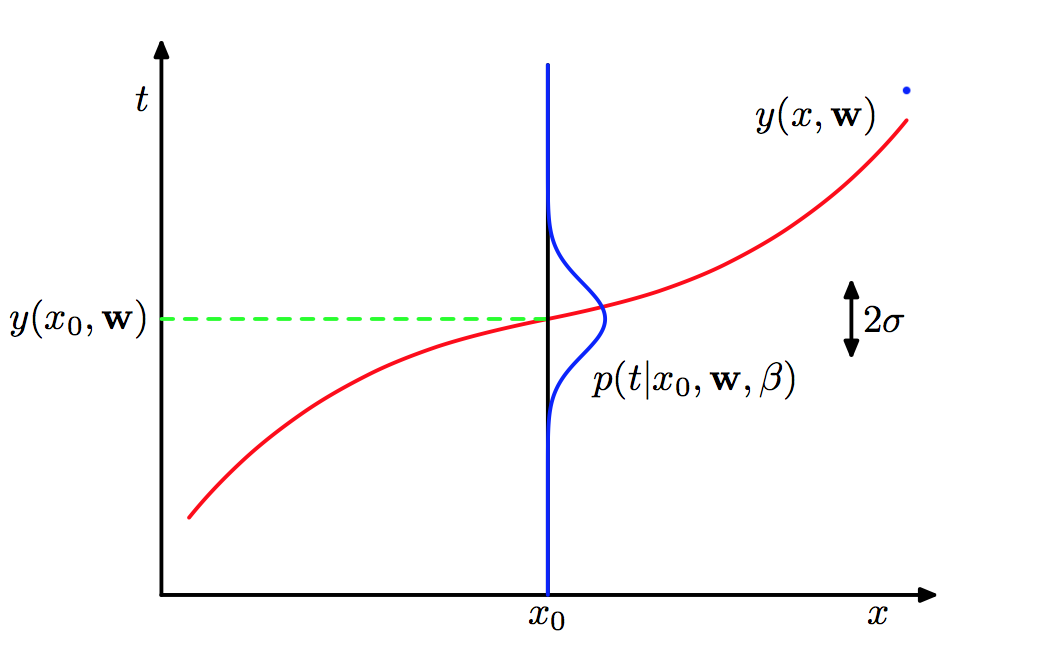
\includegraphics[width=6cm]{gaussian_conditional_poly_fitting.jpg}
        \end{center}
        Given training data $\{\matr{x}, \matr{t}\}$, we want to determine values for $\matr{w}$ and $\beta$ by maximum likelihood. The likelihood function is given by 
        \[
            p(\matr{t}|\matr{x}, \matr{w}, \beta) = 
            \prod_{n=1}^N \normal{t_n | y(x_n, \matr{w}), \beta^{-1}}    
        \]
        Maximizing likelihood is equivalent to minimizing sum-of-squares error function
        \[
            \ln{p(\matr{t}|\matr{x}, \matr{w}, \beta)}  
            = -\frac{\beta}{2} \sum_{n=1}^N (y(x_n, \matr{w}) - t_n)^2 + \frac{N}{2}\ln{\beta} -  \frac{N}{2} \ln{2\pi}  
        \]
        We can find maximum likelihood estimator $\matr{w}_{mle}$ and the corresponding precision given by 
        \[
            \frac{1}{\beta_{mle}} = \frac{1}{N}\sum_{n=1}^N (y(x_n, \matr{w}_{mle}  - t_n)^2
        \]
        Having determined parameter $\matr{w}$ and $\beta$, we can make predictions for new values of $x$ by expressing in terms of the predictive distribution. 
        \[
            p(t|x,w_{mle}, \beta_{mle})
            = 
            \normal{t|y(x,\matr{w}_{mle}, \beta^{-1}_{mle})}
        \]
        We can introduce a prior distribution over polynomial coefficients $\matr{w}$
        \[
            p(\matr{w}|\alpha) = 
            \normal{\matr{w}| \matr{0}, \alpha^{-1}\matr{I}} = 
            \left( \frac{\alpha}{2\pi} \right)^{(M+1)/2}
            \exponents{-\frac{\alpha}{2} \matr{w^Tw}}
        \]
        where $\alpha$ is precision of prior distribution and $M+1$ is the total number of elements in $\matr{w}$ for $M$th order polynomial. Also note $\matr{\Sigma}^{-1} = (\alpha^{-1}\matr{I})^{-1} = \alpha\matr{I}$. Using Bayes' theorem, we have 
        \[
            p(\matr{w}|\matr{x},\matr{t}, \alpha, \beta)
            \propto 
            p(\matr{t}|\matr{x}, \matr{w}, \beta) p(\matr{w}|\alpha)
        \]
        We can determine $\matr{w}$ by finding most probable value of $\matr{w}$ given the data, by maximizing the posterior distribution. Finding \textbf{maximum posterior} (MAP) is equivalent to minimizing negative logarithm of 
        \[
            \ln{p(\matr{w}|\matr{x},\matr{t}, \alpha, \beta)} \propto \frac{\beta}{2} \sum_{n=1}^N (y(x_n, \matr{w}) - t_n)^2 + \frac{\alpha}{2} \matr{w^Tw}    
        \]
        which is equivalent to minimize regularized sum-of-squares erorr fucntion with $\lambda = \alpha/\beta$
    \end{enumerate}
\end{defn*}

\begin{defn*}
    \textbf{Model Selection} 
    \begin{enumerate}
        \item \textbf{Motivation} Order of polynomial or regularization coefficients govern complexity of model. We want to determine the value of hyperparameters such that we achieve best predictive performance of new data. Idea is to use an independent data from \textbf{training set}, called \textbf{validation set}, and select one having the best performance. However if model is iterated many times, then some overfitting to validation data can occur., so may want to keep a third \textbf{test set} on which performance of selected model is evaluated. 
        \item \textbf{Cross-Validation} Allows proportion of $(S-1)/S$ of data to be used for training. The drwaback is 
        \begin{enumerate}
            \item Number of training runs increased by a factor of $S$, and can prove problematic for model in which the training itself is computationally expensive.
            \item If there are multiple complexity parameter in the model, exploring combinations of settings of such parameter could, in worst case, require a number of training runs that is exponential in the number of parameters. 
        \end{enumerate}
        So want to find a measure of performance which depends only on the trainin gdata and which does not suffer from bias due to overfitting. AIC/BIC are such models
    \end{enumerate}
\end{defn*}



\end{document}
